The characterization of the active shield (cosmic veto), which was carried out using PMTs as photosensors, is reported in this section. The quality of the veto wrapping was checked. As this study was done for a single photosensor, the configuration of the electronics was the one given in Figure \ref{subfig:ElectronicConfiguraiton2PMT}. The surface of the veto was divided in 9 parts, depictedin Figure \ref{fig:MappingPoints}, on which a gamma source was placed for this test. Two different tests were made for this task:

\begin{figure}[h]
\centering
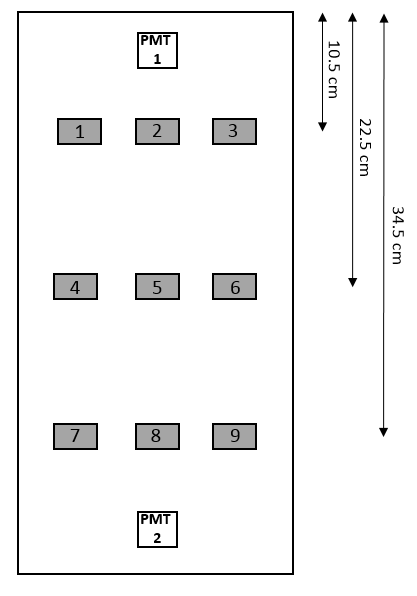
\includegraphics[scale=0.75, angle=90]{4ResearchAndDevelopments/43CosmicVetos/VetoPoints.png}
\caption{Reference points used for veto mapping.\label{fig:MappingPoints}}
\end{figure}
Two different tests were made for this task:
\begin{enumerate}

\item{} To quantify the improvement of the veto signal due to wrapping,  A $\ce{^{137}Cs}$ source was placed at point 2 before wrapping and a energy spectrum was measured with the veto. Next, the measurment was repeated after wrapping. The spectra obtained are displayed in Figure \ref{fig:VetoCoverageImprovement}.

\begin{figure}[h]
\centering
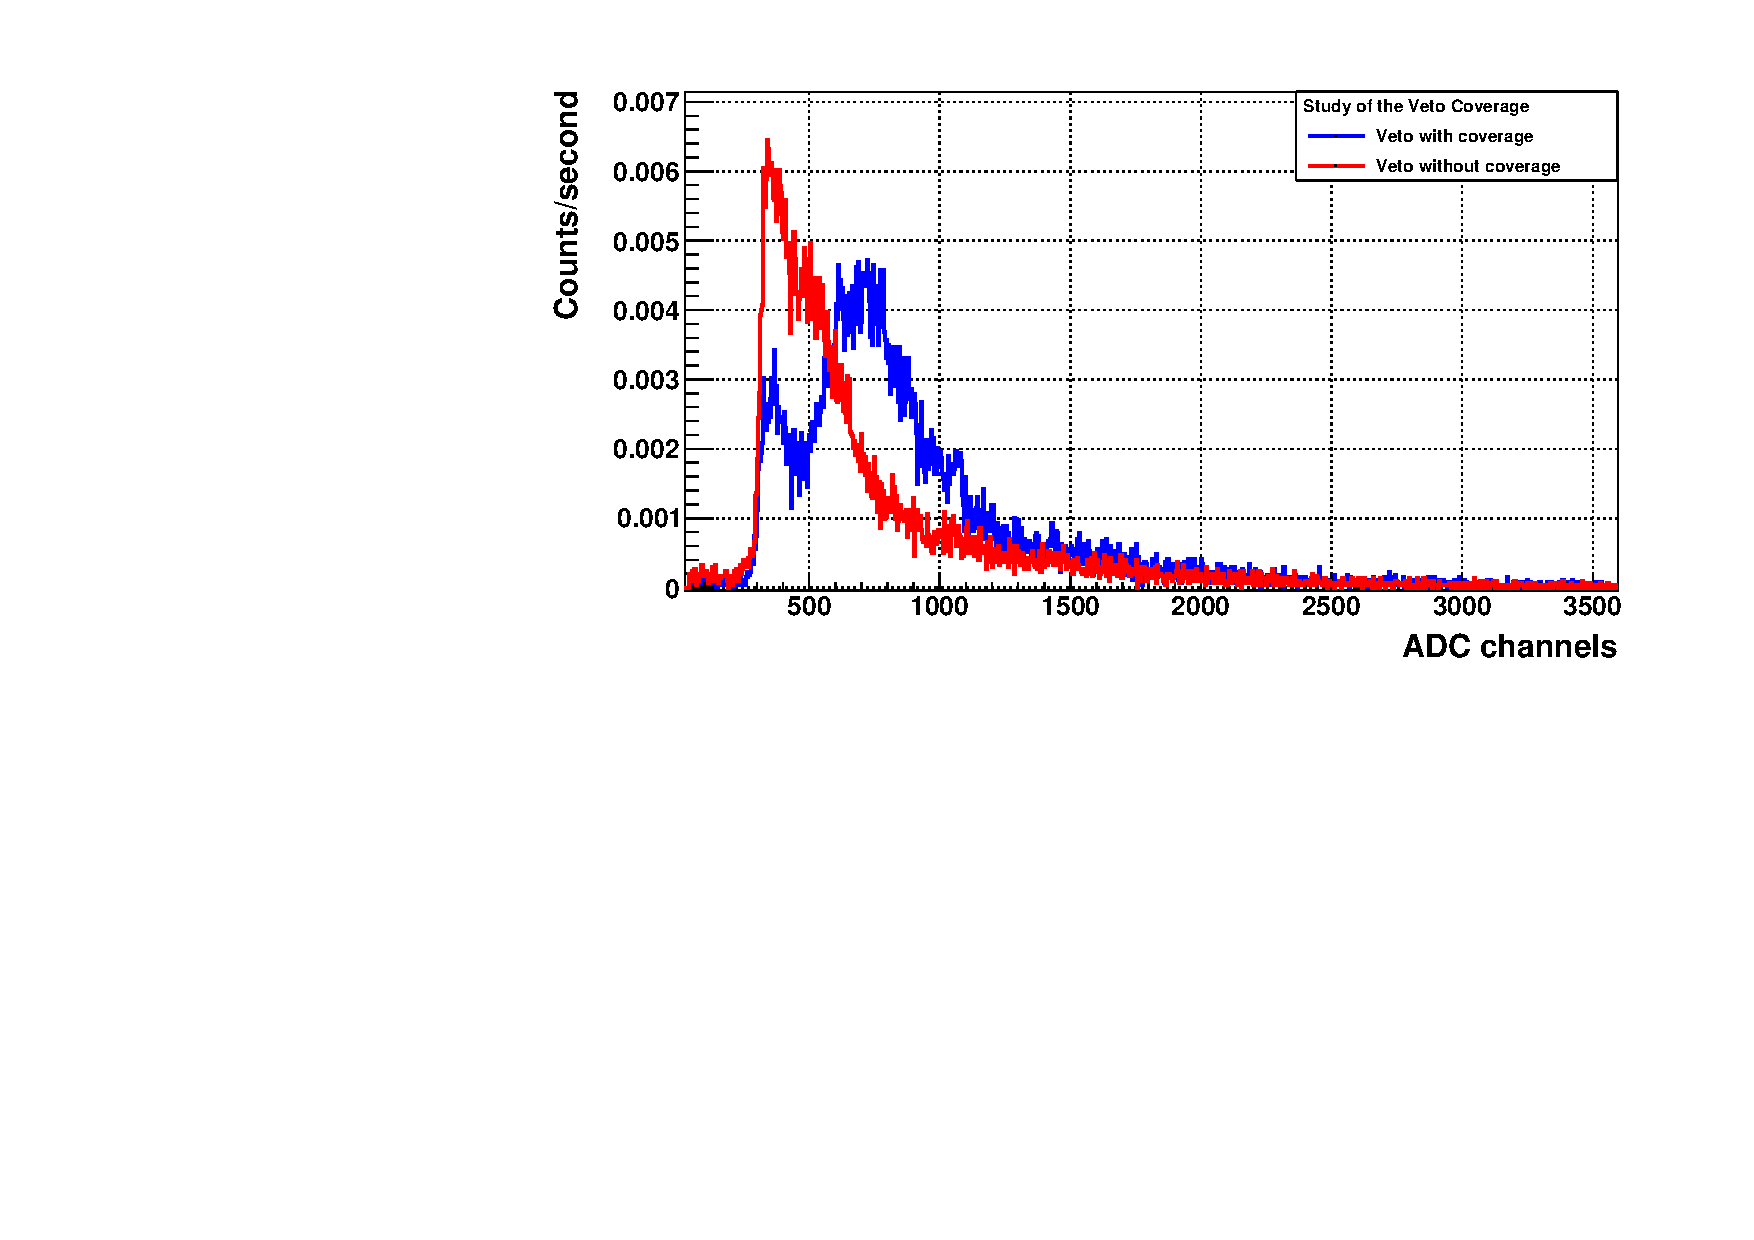
\includegraphics[scale=0.7]{4ResearchAndDevelopments/43CosmicVetos/CoverageStudy_more_rebin.pdf}
\caption{Measurement of a radioactive source $\ce{^{137}Cs}$ with the TRITIUM cosmic detector with and without wrapping.\label{fig:VetoCoverageImprovement}}
\end{figure}

The spectrum of the wrapped veto is shifted to the right, which means that more photons (a factor two) are collected. No improvement was obtained on the number of events detected, only on the collection efficiency.

%a comparison is made between the measurement of cover and uncover veto, placing the gamma source in 3 different points, 1, 2 and 3. This study is used 

\item{} The spatial uniformity of the signal of the wrapped veto was evaluated. For this task, a mapping of the response of a $\ce{^{60}Co}$ source on each test point was done for two different veto modules and the energy spectra obtained were integrated. The count rates obtained are plotted in Figure \ref{fig:MappingVetos}. It can be observed that the veto signal has a uniform response on its whole surface, giving a fairly similar counting rate at all the points.
%\begin{table}[htbp]
%%\centering
%\begin{center}
%\begin{tabular}{|c|c|c|}
%\hline
%Point & Veto 1 (counts/s) & Veto 2 (counts/s)\\
%\hline \hline \hline
%1 & $18028\pm 3$ & $18293 \pm 1.5$ \\ \hline
%2 & $19133 \pm 5$ & $20014 \pm 4$  \\ \hline
%3 & $17858 \pm 4$ & $18843 \pm 4$  \\ \hline
%4 & $18969 \pm 5$ & $18761 \pm 5$  \\ \hline
%5 & $19893 \pm 4$ & $19841 \pm 3$  \\ \hline
%6 & $18573 \pm 4$ & $18850 \pm 5$  \\ \hline
%7 & $18200 \pm 4$ & $17790 \pm 4$  \\ \hline
%8 & $19725 \pm 4$ & $19312 \pm 4$  \\ \hline
%9 & $18030 \pm 5$ & $17804 \pm 5$  \\ \hline
%\end{tabular}
%\caption{Count rate measured with two different cosmic detectors using a radioactive source $\ce{^{60}Co}$.}
%\label{tab:MappingDataVetos}
%\end{center}
%\end{table}
\begin{figure}
\centering
    \begin{subfigure}[b]{0.9\textwidth}
    \centering
    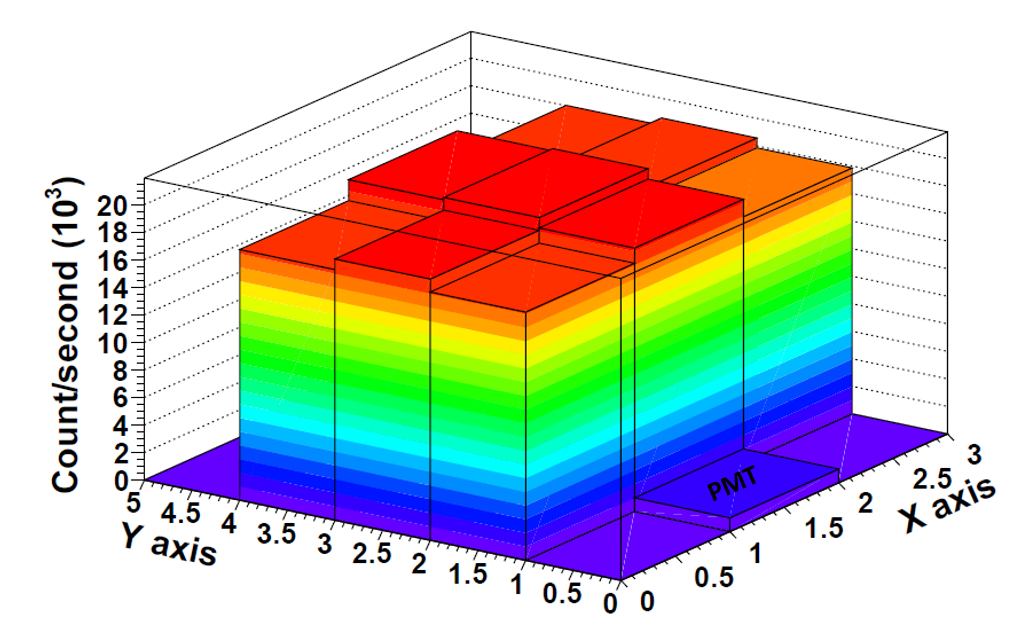
\includegraphics[width=\textwidth]{4ResearchAndDevelopments/43CosmicVetos/MappingVeto1.png}  
    \caption{\label{subfig:MappingVeto1}}
    \end{subfigure}
    \hfill
    \begin{subfigure}[b]{0.9\textwidth}
    \centering
    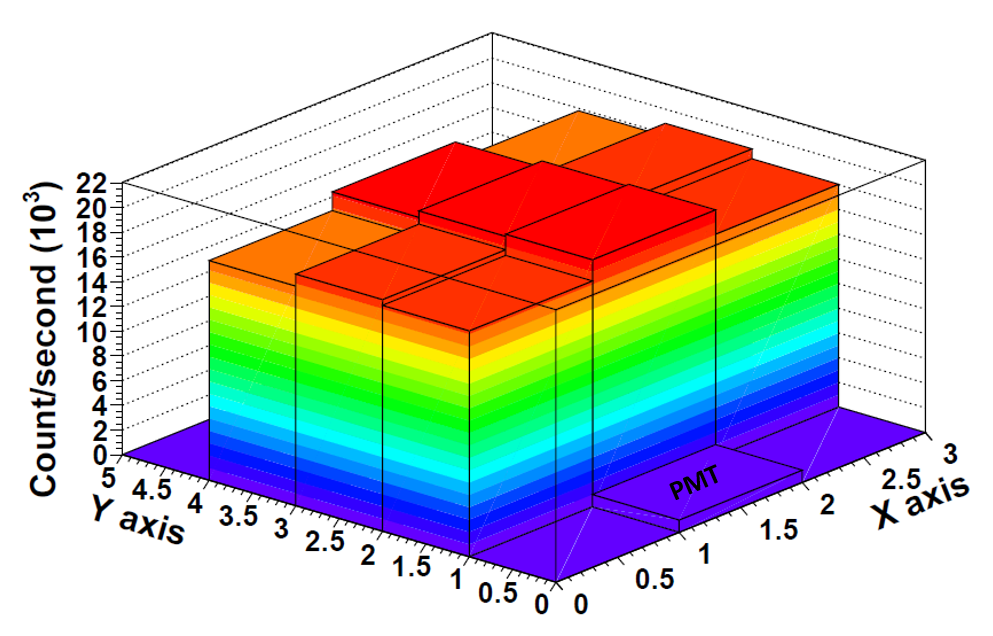
\includegraphics[width=\textwidth]{4ResearchAndDevelopments/43CosmicVetos/MappingVeto2.png}  
    \caption{\label{subfig:MappingVeto2}}
    \end{subfigure}
 \caption{Bidimensional graph of the counting rate (mapping) measured for two different TRITIUM cosmic detectors using a $\ce{^{60}Co}$ source.}
 \label{fig:MappingVetos}
\end{figure}
\end{enumerate}

Next, both vetos in time coincidence were studied with the configuration of the electronics of Figure \ref{subfig:ElectronicConfiguraiton4PMT}. The goal was to find the conditions of which the detection of cosmic rays is optimized. This optimization consisted of the lowest PMT high voltage at which the veto efficiency is stable and the highest discriminator threshold that produces no loss of cosmic events. For higher voltages and a smaller thresholds, a plateau of the counting rate should be obtained. The counting rate was measured for several high voltages at fixed threshold and for several thresholds at fixed high voltage. The results are plotted in Figure \ref{fig:HVandThresholdsPLateaus}. To find the optimal conditions, the amplification line of the electronics was eliminated and the output signal of the coincidence module was connected to a 1145 CAEN Quad Scaler And Preset Counter-Timer module \cite{ScalerDataSheet}. The counting rate was measured in a time window of $300~\second$. In Figure \ref{subfig:HVPLateauVetos}, the counting rate at several high voltages for three different thresholds, $60~\milli\volt$, $100~\milli\volt$ and $200~\milli\volt$ is plotted. As it can be observed, there is a minimum high voltage for each threshold, $700~\volt$, $730~\volt$ and $780~\volt$ respectively, at which the plateau start. This minimum voltage is higher when the value of the threshold increases, as it should. Analogously, the counting rate was measured for $750~\volt$, $800~\volt$ and $850~\volt$ HV, shown in Figure \ref{subfig:ThresholdsPlateau} finding that the plateau ends at $140~\milli\volt$, $270~\milli\volt$ and $450~\milli\volt$ respectively. This maximum threshold increases with high voltage, as it should. The voltage chosen was $800~\volt$ since it is on the plateau for the three thresholds and the threshold chosen was $200~\milli\volt$ which is on the plateau for the selected high voltage. 
\begin{figure}
\centering
    \begin{subfigure}[b]{0.8\textwidth}
    \centering
    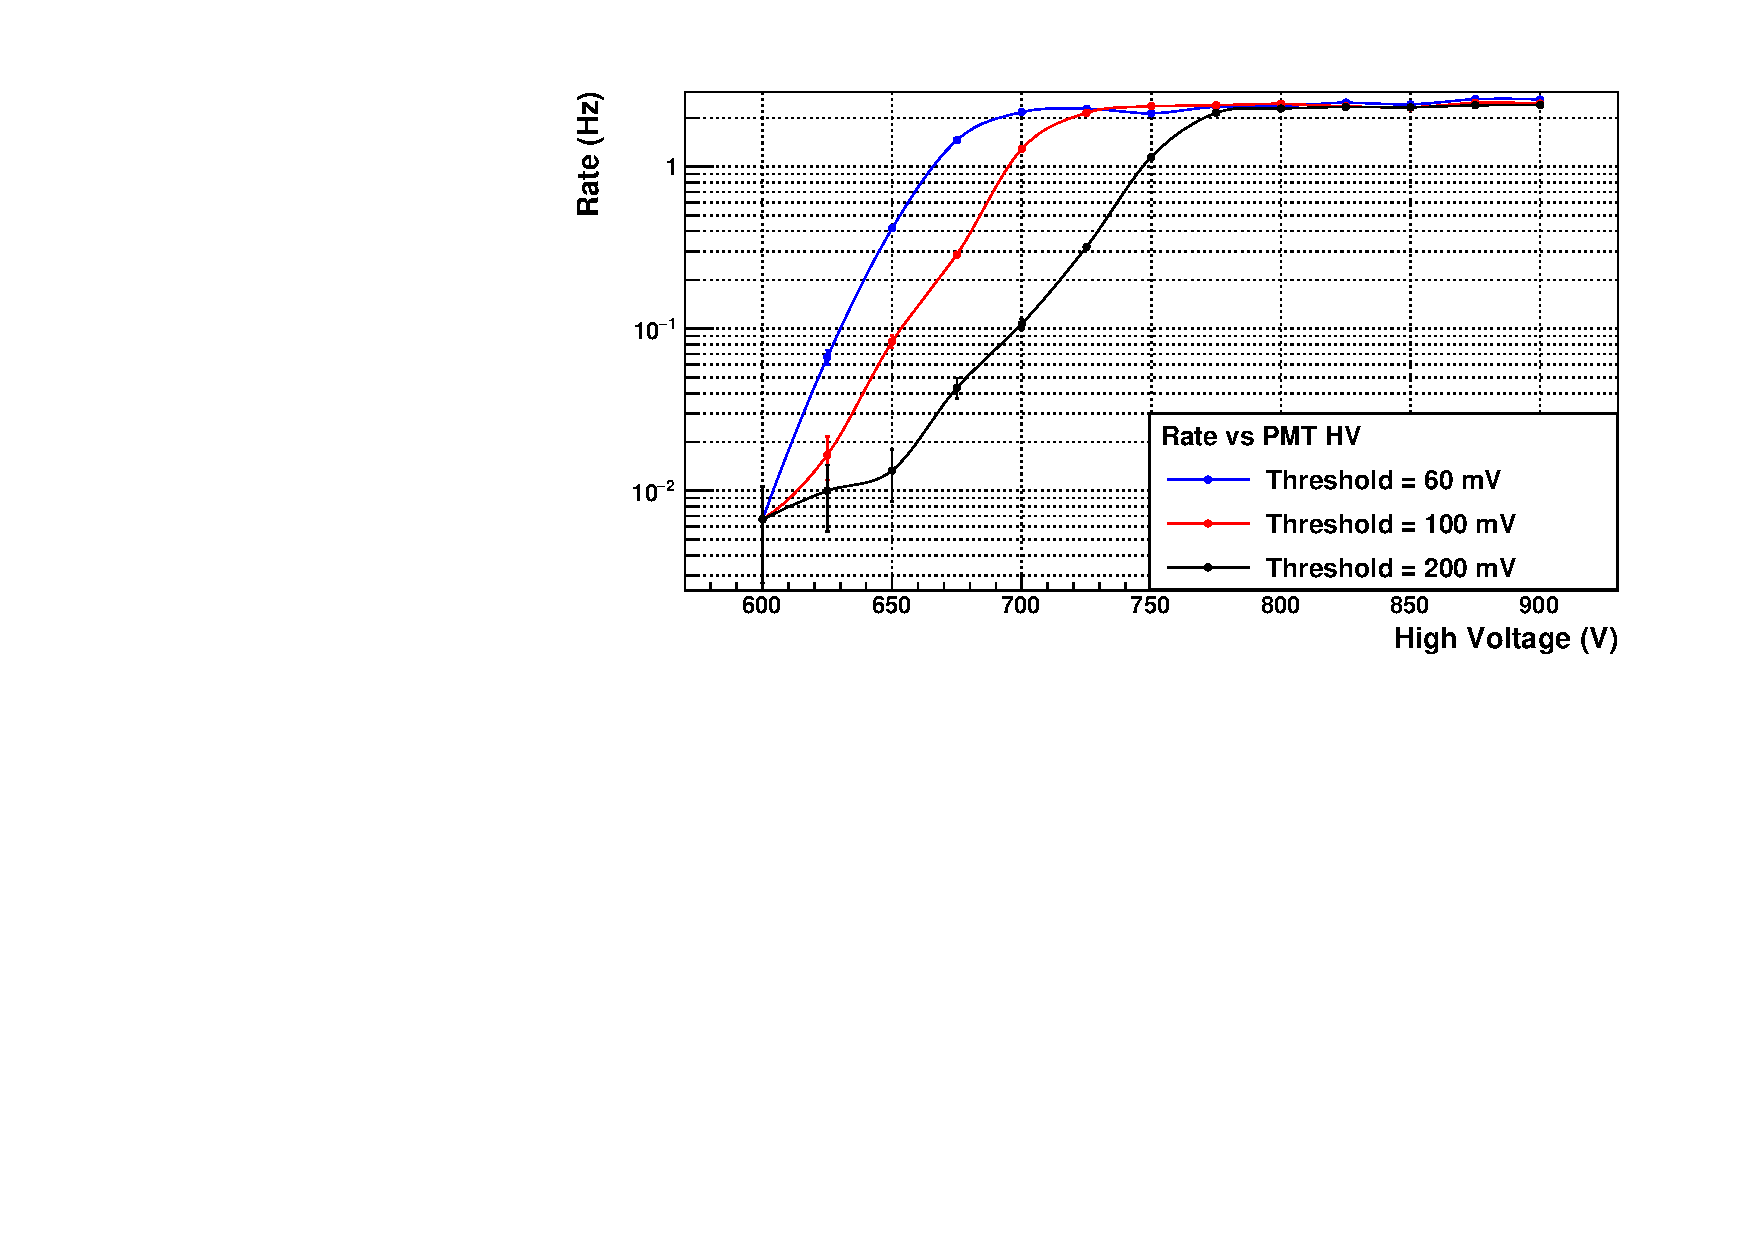
\includegraphics[width=\textwidth]{4ResearchAndDevelopments/43CosmicVetos/Counts_for_several_HV_VETOS.pdf}  
    \caption{\label{subfig:HVPLateauVetos}}
    \end{subfigure}
    \hfill
    \begin{subfigure}[b]{0.8\textwidth}
    \centering
    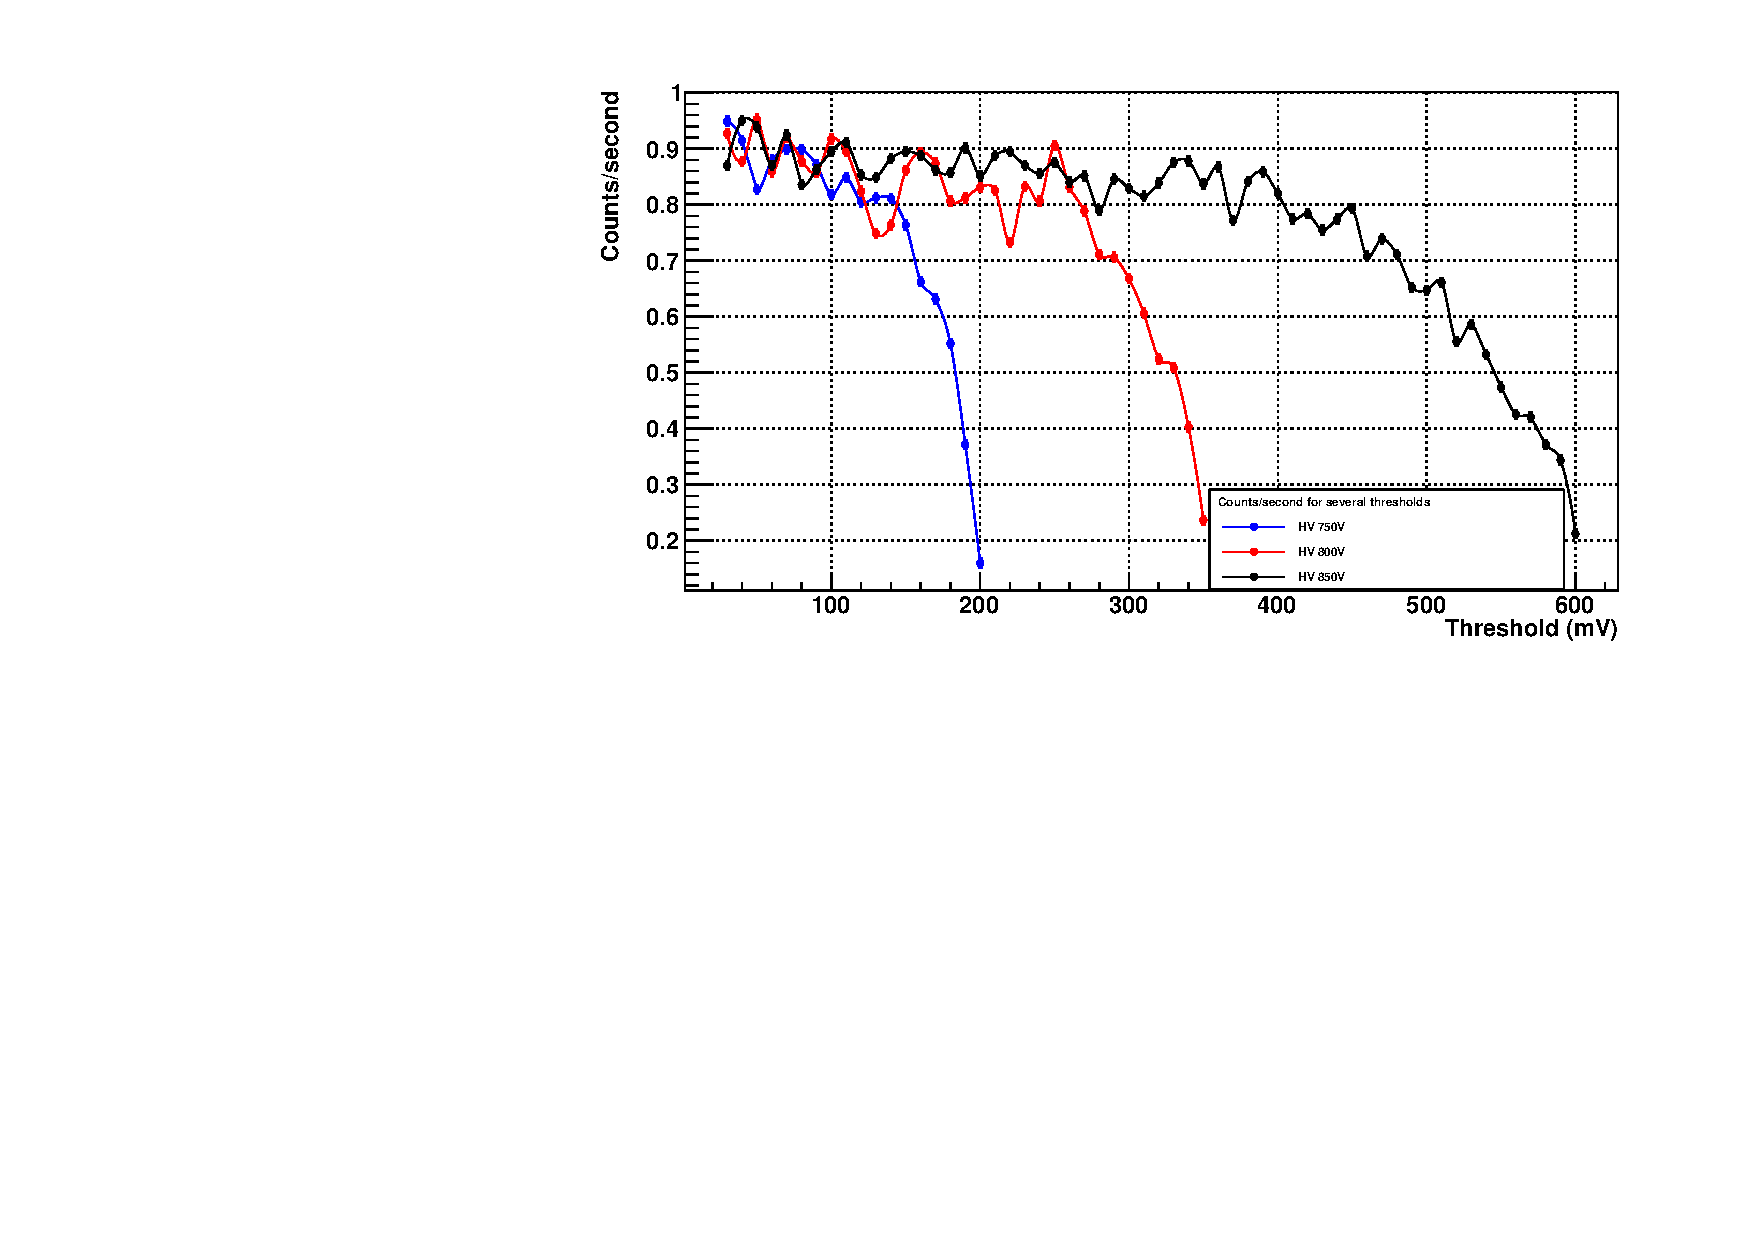
\includegraphics[width=\textwidth]{4ResearchAndDevelopments/43CosmicVetos/Counts_for_several_thresholds_VETOS.pdf}  
    \caption{\label{subfig:ThresholdsPlateau}}
    \end{subfigure}
 \caption{ Veto counting rate (semilogaritmic scale) a) as a function of HV for a fixed threshold and b) as function of threshold for fixed high voltage.}
 \label{fig:HVandThresholdsPLateaus}
\end{figure}
With this setting, the energy spectrum of cosmic events was measured, shown in Figure \ref{fig:EnergySpectrumCosmicVeto}. 
\begin{figure}[h]
\centering
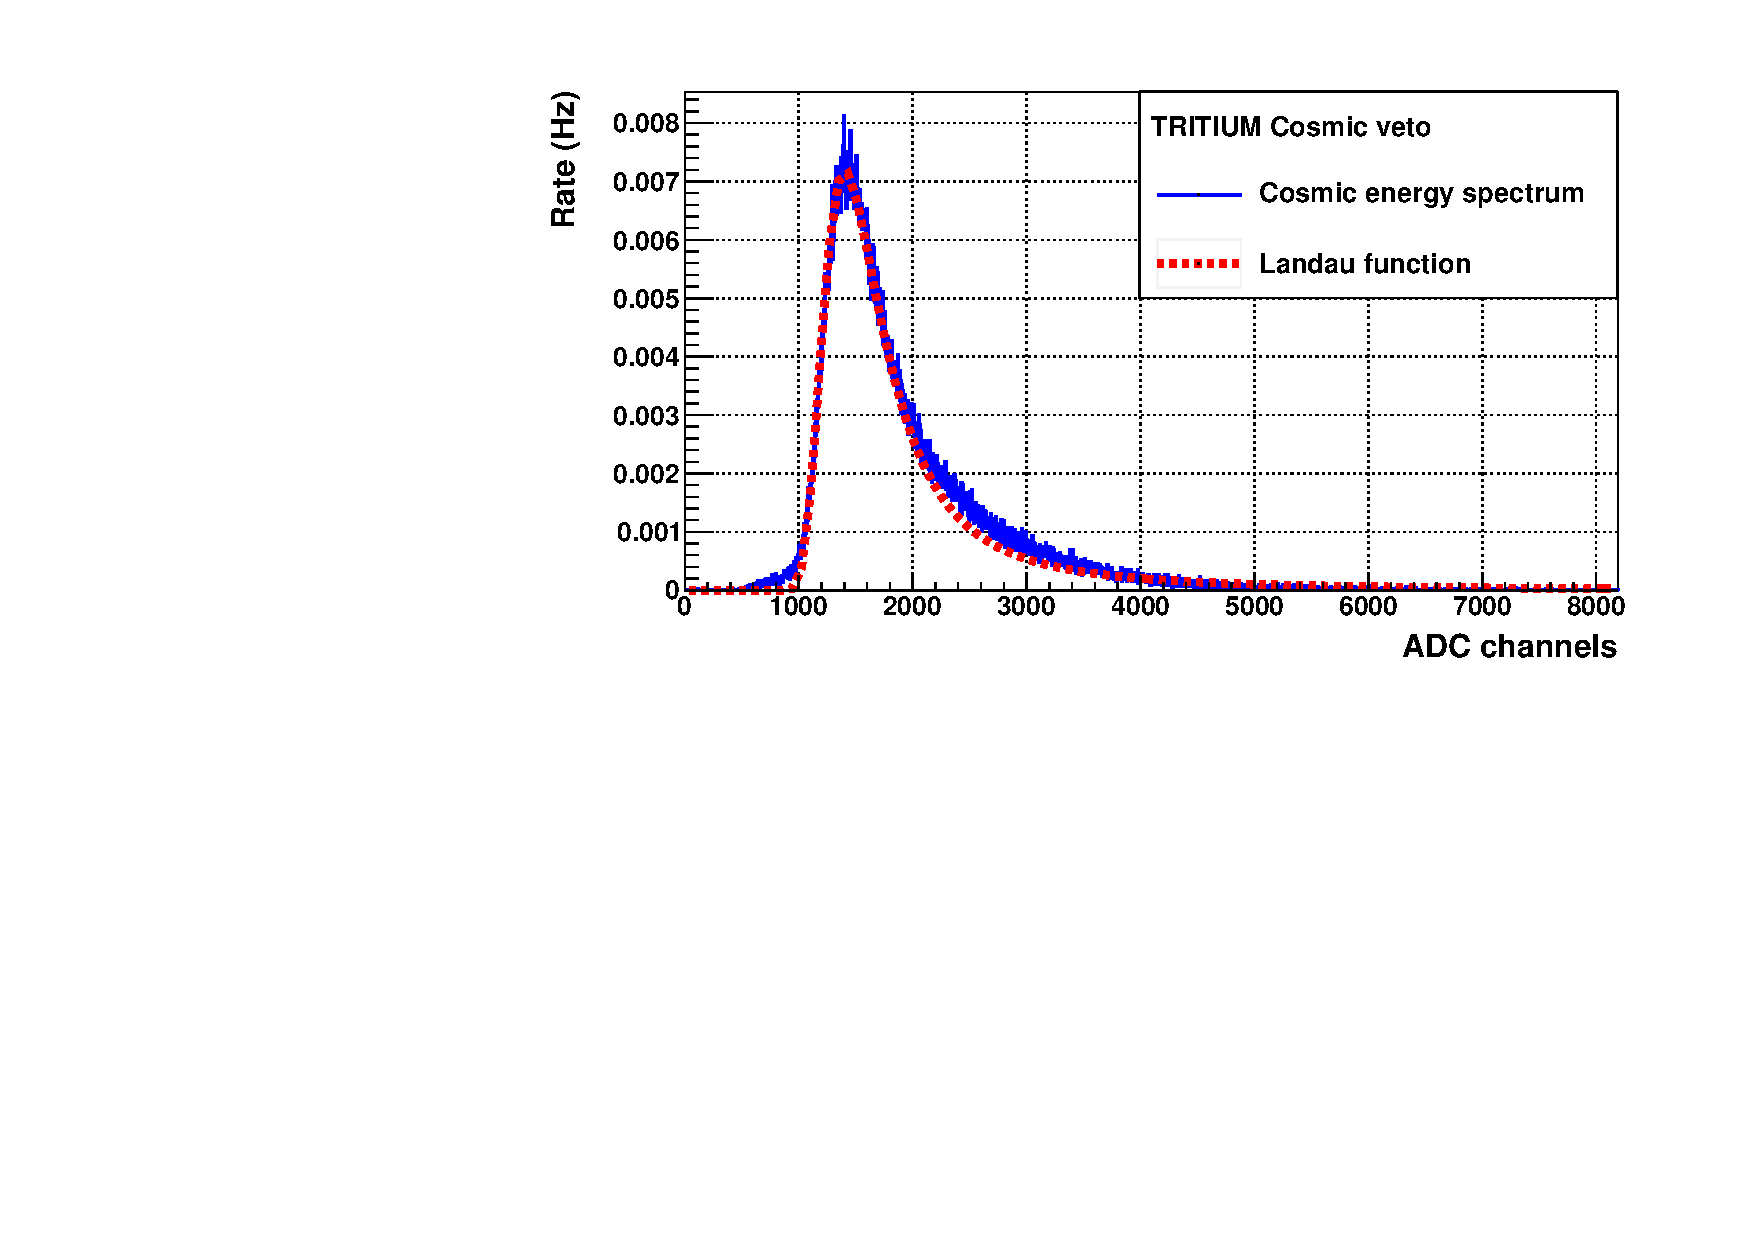
\includegraphics[scale=0.6]{4ResearchAndDevelopments/43CosmicVetos/Cosmic_Energy_Spectrum_36_cm_Landau_Function.pdf}
\caption{Energy spectrum measured with the cosmic veto.\label{fig:EnergySpectrumCosmicVeto}}
\end{figure}
As expected, this energy spectrum fits well to a Landau function. The cosmic ray rate determined from the area of this spectrum is $2.5~$event$/\second$. The expected cosmic rate, calculated in section \ref{subsec:SetUpActiveShield}, is $2.9~$event$/\second$, so the efficiency of the active veto is $85\%$, which is a usual value of the efficiency of plastic detectors for mips. Finally the detected cosmic ray rate versus the separator distance between the two cosmic vetos was obtained. The energy spectrum was measured for several distances. The spectra are plotted in Figure \ref{subfig:EnergySpectrumsSeveralDistanceVeto}. The counting rate decreases with the distance but the spectrum shape remains the same. The integrated spectra as a function of distance, plotted in Figure \ref{subfig:LinearFitSeveralDistanceVeto}, was fitted to a second degree polynomial. The fits allows us to estimate the cosmic rate for a given veto distance.

%As can be seen, the shape of the spectrum is the same because the energy of the detected events is the same (cosmic events) but the quantity of their events is less for greater distance. The reason for that is that when the distance is increased, the solid angle formed by the active veto is smaller.

%The detected cosmic events was calculated by the area integral and they are represented in Figure \ref{subfig:LinearFitSeveralDistanceVeto} as a function of the distance between both detectors, where a linear fit has been added. With this linear fit, the detected cosmic rate can be easily known if the working distance is changed. 

%\begin{figure}[htbp]
%\centering
%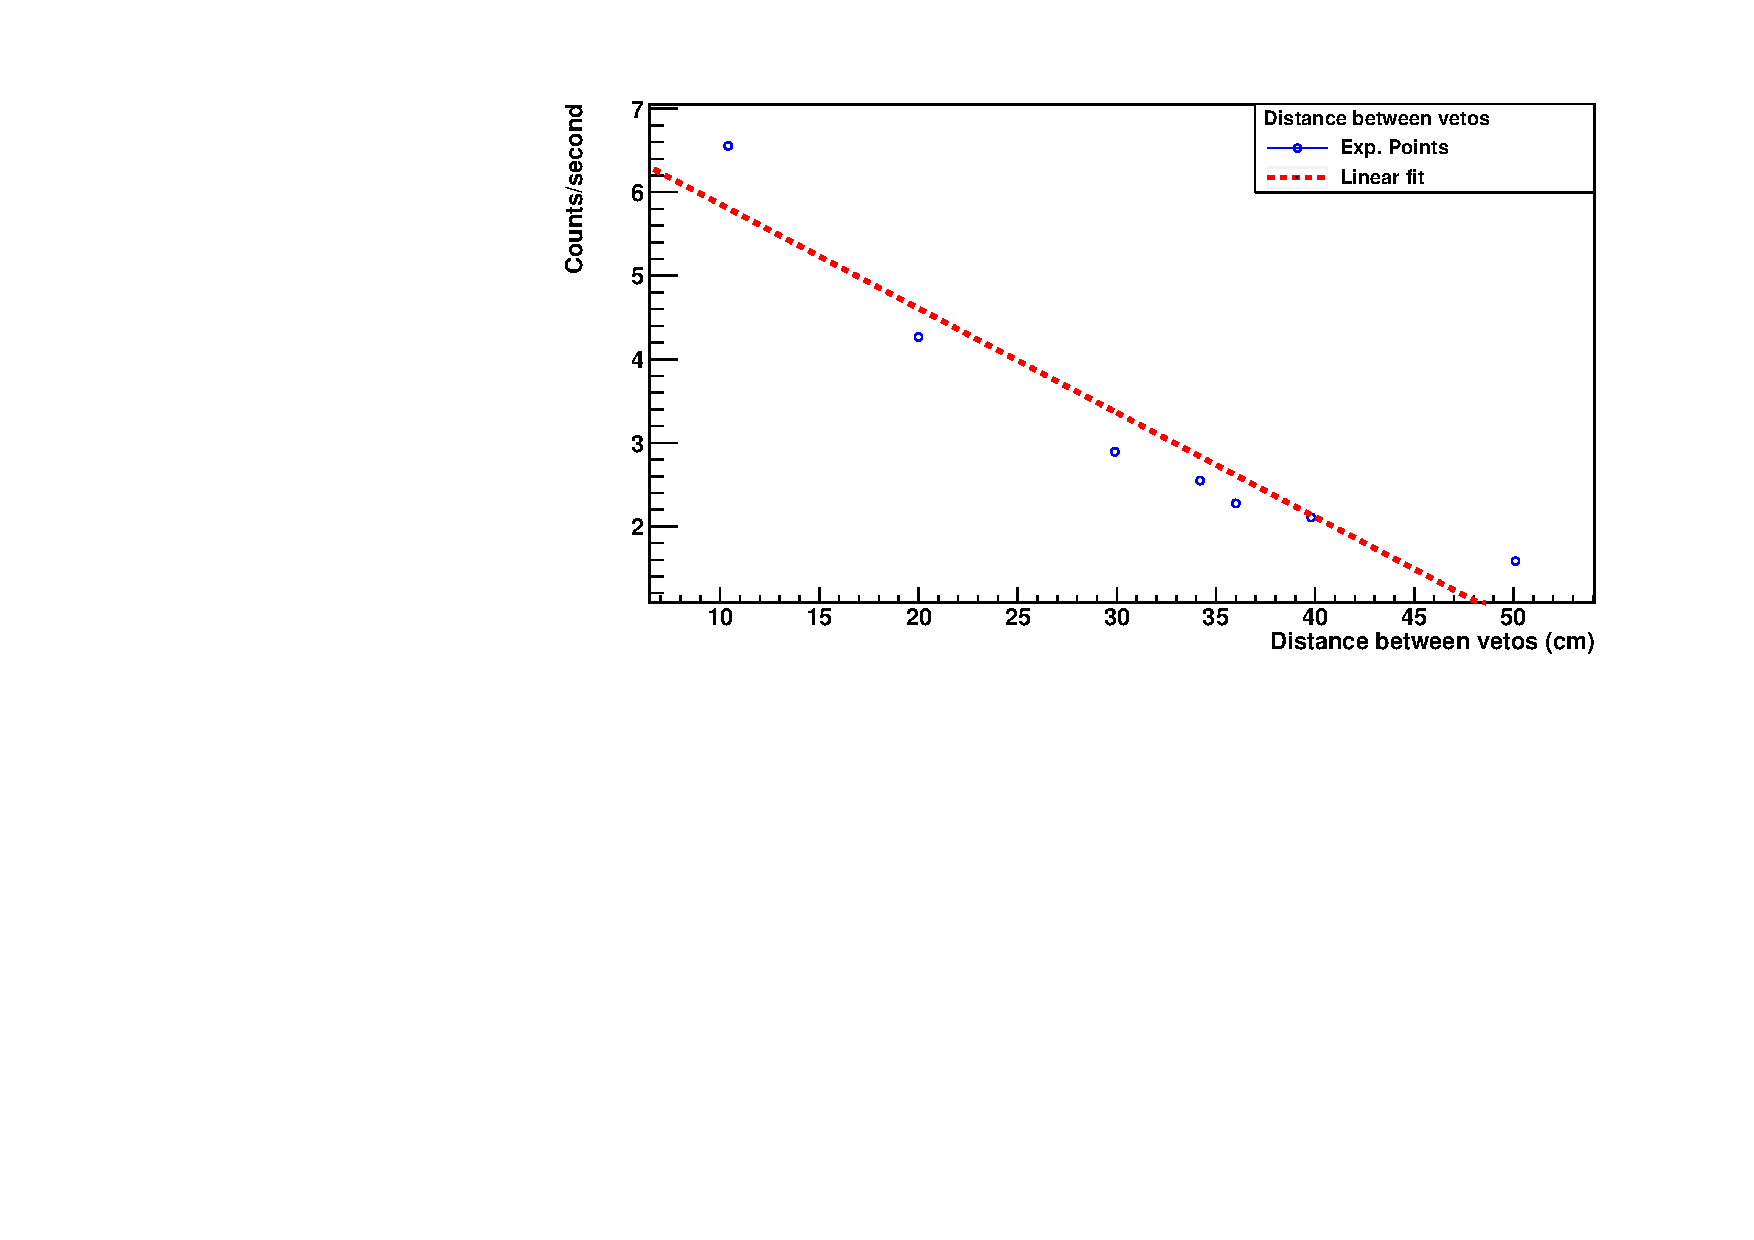
\includegraphics[scale=0.6]{4ResearchAndDevelopments/43CosmicVetos/LinearFit_SeveralDistance_Veto.pdf}
%\caption{Linear fit of the counts per second measured with the cosmic veto with several distance between its cosmic detectors.\label{fig:LinearFitSeveralDistanceVeto}}
%\end{figure}


\begin{figure}
\centering
    \begin{subfigure}[b]{0.85\textwidth}
    \centering
    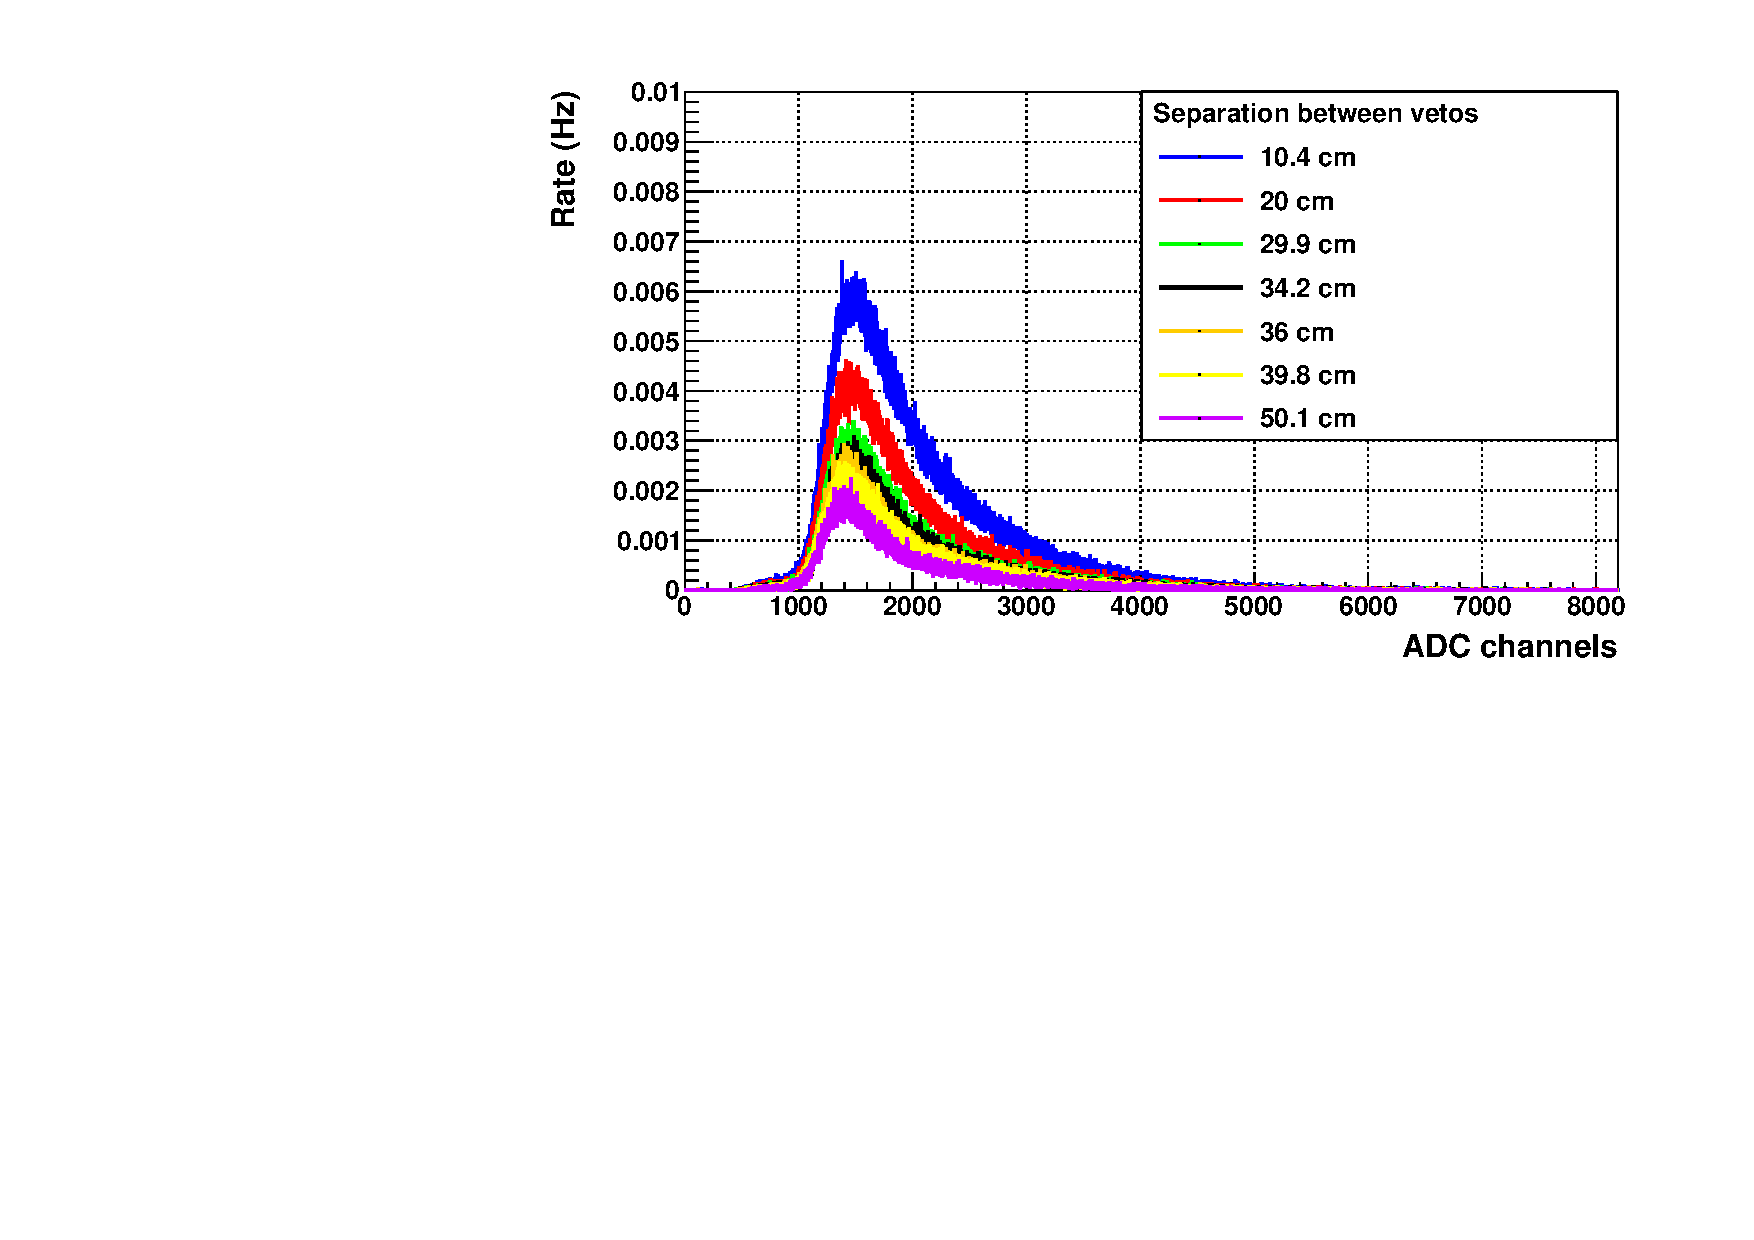
\includegraphics[width=\textwidth]{4ResearchAndDevelopments/43CosmicVetos/Energy_Plots_SeveralDistance_Veto.pdf}  
    \caption{\label{subfig:EnergySpectrumsSeveralDistanceVeto}}
    \end{subfigure}
    \hfill
    \begin{subfigure}[b]{0.85\textwidth}
    \centering
    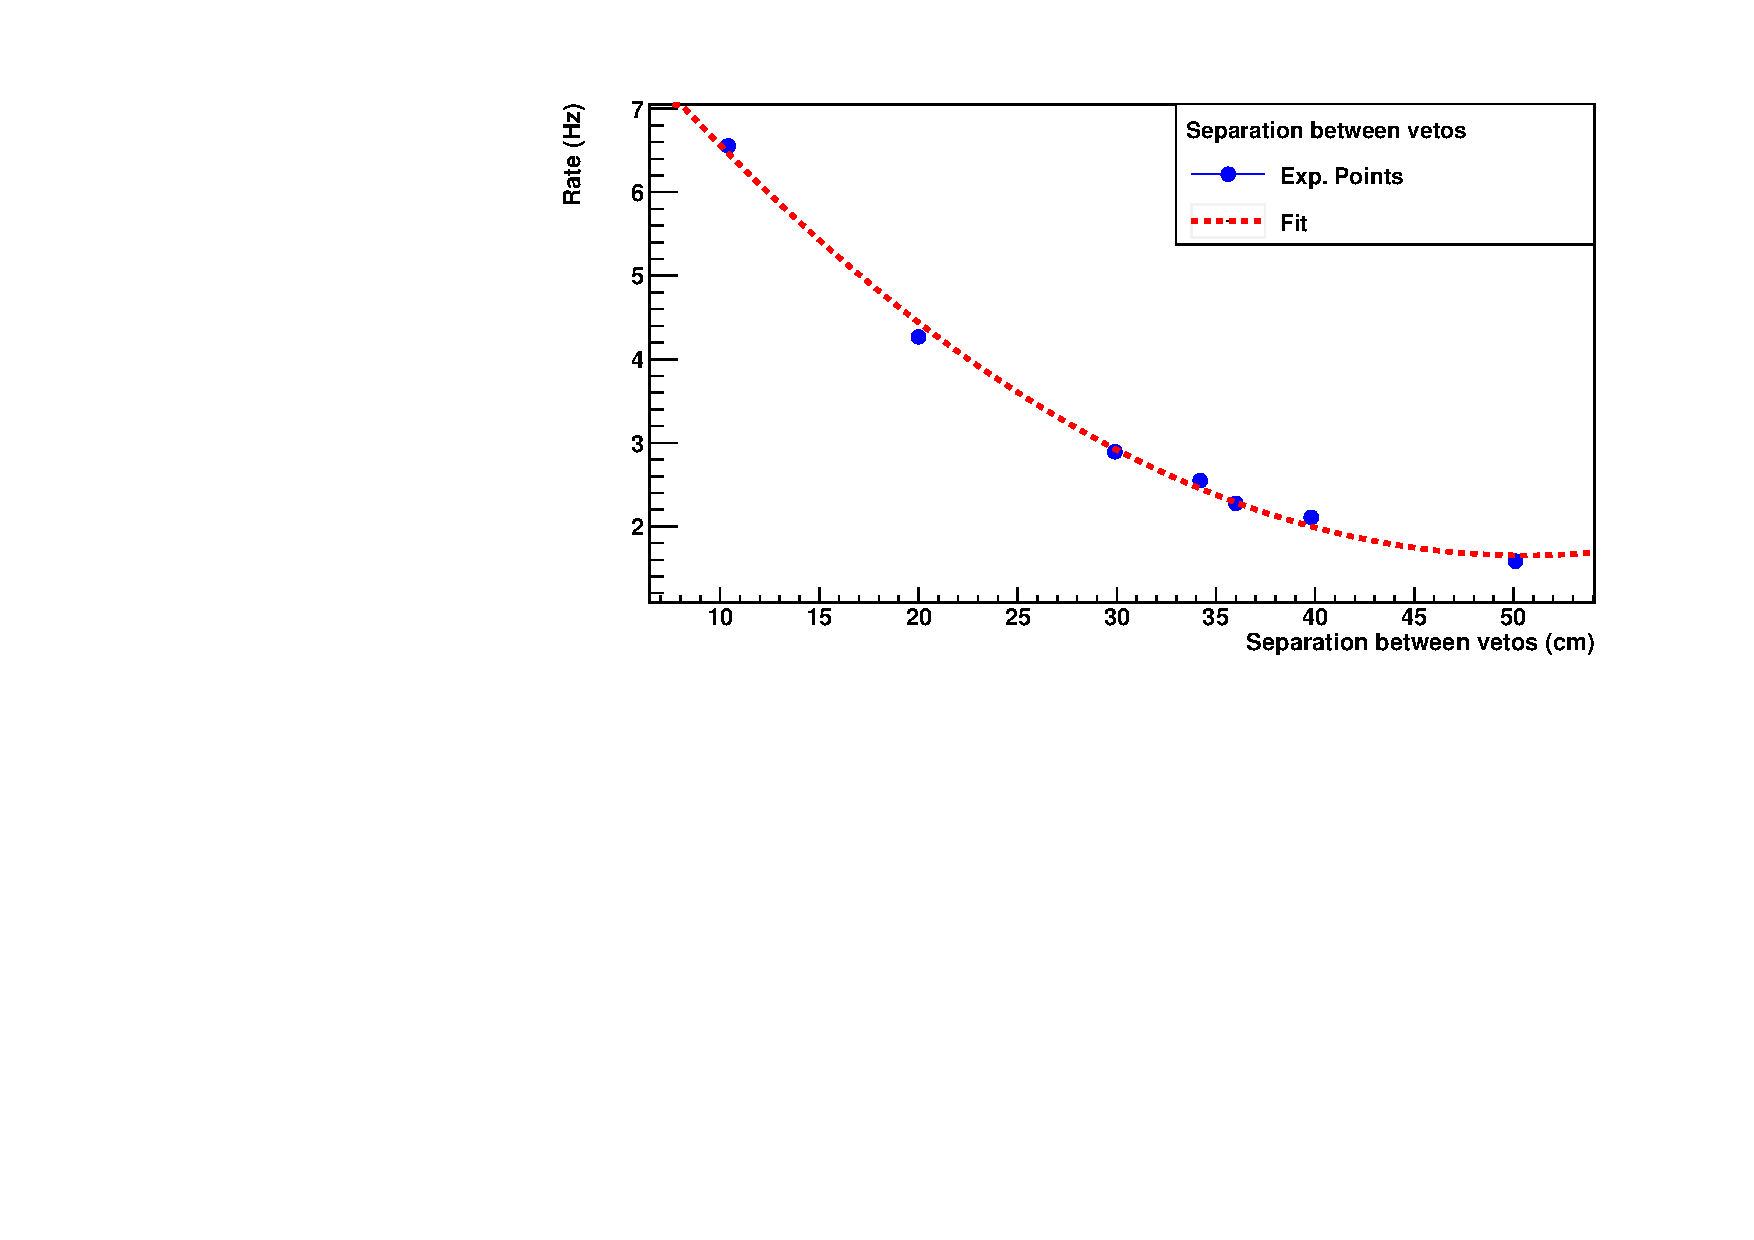
\includegraphics[width=\textwidth]{4ResearchAndDevelopments/43CosmicVetos/Pol2Fit_SeveralDistance_Veto.pdf}  
    \caption{\label{subfig:LinearFitSeveralDistanceVeto}}
    \end{subfigure}
 \caption{a) Energy spectra of the cosmic veto for several separator distances of the scintillators. b) Fit of the cosmic veto rate versus the separator distance of the scintillators to a second degree polynomial.}
 \label{fig:DistanceVeto}
\end{figure}
%También se realizaron varias medias para ver como afecta una fuente gama. Discutir con Pepe como plantear esta medida o si merece la pena ponerla o no.

%Como es de esperar esta deja muy poca señal en el centelleador ya que este tiene muy poca eficiencia para gammas.